\usetikzlibrary{positioning,shapes,shadows,arrows,calc,matrix,backgrounds,decorations.pathreplacing}
\tikzset{note/.style={rectangle callout, rounded corners,fill=gray!20,drop shadow,font=\footnotesize}}    

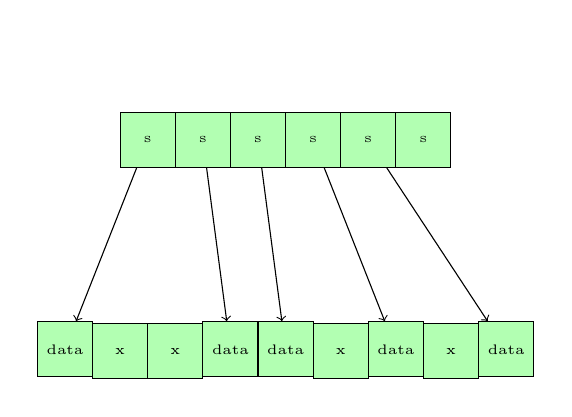
\begin{tikzpicture}[font=\ttfamily,
 vector/.style={matrix of nodes,nodes={draw, minimum size=7mm, fill=green!30},
            column sep=-\pgflinewidth, row sep=0.0mm, nodes in empty cells, font=\tiny,
            row 1/.style={nodes={draw=none, fill=none}}}]
            
            \matrix[vector, label={}] (vec) {
                \\s & s & s & s & s & s \\};
            %\element{3,4,7,9}{red!30}
            \matrix[vector, below=of vec, label={}] (mem) {
                \\data & x & x & data & data & x & data & x & data \\};
			\draw[->](vec-2-1) -- (mem-2-1);
			\draw[->](vec-2-2) -- (mem-2-4);
			\draw[->](vec-2-3) -- (mem-2-5);
			\draw[->](vec-2-4) -- (mem-2-7);
			\draw[->](vec-2-5) -- (mem-2-9);
\end{tikzpicture}